\documentclass[pdflatex]{sn-jnl}
\renewcommand{\textfraction}{.002}
\renewcommand{\floatpagefraction}{.995}
\setcounter{totalnumber}{5}
\renewcommand{\topfraction}{.995}

\usepackage[numbers,square]{natbib}
\bibliographystyle{spbasic_u}

\usepackage[noend,ruled,vlined]{algorithm2e}
\newcommand\mycommfont[1]{\footnotesize\ttfamily{#1}}
\SetCommentSty{mycommfont}


\usepackage{graphicx}%
\usepackage{multirow}%
\usepackage{amsmath,amssymb,amsfonts}%
\usepackage{amsthm}%
\usepackage{mathrsfs}%
\usepackage[title]{appendix}%
\usepackage{xcolor}%
\usepackage{textcomp}%
\usepackage{manyfoot}%
\usepackage{booktabs}%
\usepackage{placeins}
\usepackage{listings}%
\usepackage{mathtools}
\usepackage{subcaption}
\usepackage{xr}
\usepackage{bm}
\usepackage{xfrac}
%% CUSTOM PACKAGES
%\usepackage[linesnumbered,ruled,vlined]{algorithm2e}
\usepackage{hyperref}
\usepackage{array}
\usepackage{tabularx}
\usepackage{tikz}
\usetikzlibrary{shapes.geometric}
%\usetikzlibrary{3d,perspective}
%\usetikzlibrary{shapes.geometric, arrows.meta, positioning}
\usepackage{booktabs} % For better table lines
\usepackage[version=4]{mhchem} 
\usepackage{enumitem}
\usepackage{algorithm2e}
%\usepackage{arydshln}

%%%%%%%%%%%%%%%%%%%%%%%%%%%%%%%%%%%%%%%%%%%%%%%%%%%%%%%%%%%%%%%%%%%%%%%%%%%

%% as per the requirement new theorem styles can be included as shown below
\theoremstyle{thmstyleone}%
\newtheorem{theorem}{Theorem}%  meant for continuous numbers
\newtheorem{corollary}[theorem]{Corollary}% 
\newtheorem{proposition}[theorem]{Proposition}%
\newtheorem{lemma}[theorem]{Lemma}% 
\newtheorem{conjecture}[theorem]{Conjecture}%
\newtheorem{observation}[theorem]{Observation}%
%
\makeatletter
\newtheoremstyle{examplesty}% Numbered
{18pt plus2pt minus1pt}% Space above
{18pt plus2pt minus1pt}% Space below
{\normalfont}% Body font
{0pt}% Indent amount
{\bfseries}% Theorem head font
{.}% Punctuation after theorem head
{.5em}% Space after theorem headi
{\thmname{#1}\thmnumber{\@ifnotempty{#1}{ }{#2}}%
  \thmnote{ {\the\thm@notefont(#3)}}}% Theorem head spec (can be left empty, meaning `normal')
\makeatother
\theoremstyle{examplesty}%
\newtheorem{example}{Example}%
%\newtheorem{remark}{Remark}%
%
\theoremstyle{thmstylethree}%
\newtheorem{definition}[theorem]{Definition}%

%%%%% SOME LOW LEVEL STUFF NEEDED FOR SPECIAL SYMBOLS
\makeatletter
\def\moverlay{\mathpalette\mov@rlay}
\def\mov@rlay#1#2{\leavevmode\vtop{%
    \baselineskip\z@skip \lineskiplimit-\maxdimen
    \ialign{\hfil$\m@th#1##$\hfil\cr#2\crcr}}}
\newcommand{\charfusion}[3][\mathord]{
  #1{\ifx#1\mathop\vphantom{#2}\fi
    \mathpalette\mov@rlay{#2\cr#3}
  }
  \ifx#1\mathop\expandafter\displaylimits\fi}
\DeclareRobustCommand\bigop[1]{%
  \mathop{\vphantom{\sum}\mathpalette\bigop@{#1}}\slimits@
}
\newcommand{\bigop@}[2]{%
  \vcenter{%
    \sbox\z@{$#1\sum$}%
    \hbox{\resizebox{\ifx#1\displaystyle.9\fi\dimexpr\ht\z@+\dp\z@}{!}{$\m@th#2$
}}%
  }%
}
\makeatother
%%%%% END LOWLEVEL USER DEFINITION

\newcommand{\cupdot}{\charfusion[\mathbin]{\cup}{\cdot}}
\DeclareMathOperator{\bigcupdot}{\charfusion[\mathop]{\bigcup}{\cdot}}
% \DeclareMathOperator{\Aut}{Aut}
% \DeclareMathOperator{\orb}{orb}
\newcommand{\whatever}{\mbox{\,.\,}}
\newcommand{\king}{K}
\newcommand{\queen}{\mathbf{Q}}
\newcommand{\princess}{\mathbf{P}}
\newcommand{\lord}{L}
\newcommand{\food}{\ensuremath{\mathbf{F}}}
\newcommand{\SM}{S}
\newcommand{\CRS}{\ensuremath{\mathbf{\Phi}}}
\newcommand{\closure}[2]{\mathscr{C}_{#1}(#2)}
\newcommand{\cl}[0]{c}
\newcommand{\CR}[0]{\mathcal{R}}
\newcommand{\C}[1]{\mathit{#1}}
\newcommand{\FR}[0]{\mathbf{R}}
\newcommand{\RGraph}[0]{\mathcal{R}}
%\newcommand{\F}[1]{\mathbf{#1}}
\newcommand{\fr}[0]{\mathbf{r}}
\newcommand{\crnr}[0]{\textit{r}}
\newcommand{\net}[1]{\hat{#1}}
\newcommand{\RAF}[0]{\mathbf{R}'}
\newcommand{\block}[0]{\mathbf{B}}
\newcommand{\PO}[0]{d}
\newcommand{\POR}[0]{\mathscr{R}}
\newcommand{\POX}[0]{\mathscr{X}}
\newcommand{\cat}{\kappa_F}
\newcommand{\sgen}{g}
\newcommand{\rgen}{\gamma}
\newcommand{\crgen}{\delta}
\newcommand{\ceducts}{\rho}
\newcommand{\cproducts}{\pi}
\newcommand{\feducts}{\rho_F}
\newcommand{\nfeducts}{\hat{\rho}_F}
\newcommand{\fproducts}{\pi_F}
\newcommand{\nfproducts}{\hat{\pi}_F}
\newcommand{\ORCID}[1]{}
\DeclareMathOperator{\suck}{succ}
\newcommand{\Code}[1]{\texttt{\upshape{#1}}}
\newcommand{\pfad}[0]{\ensuremath{\mathbf{P}}}
\newcommand{\stack}[0]{\ensuremath{\mathbf{T}}}
\newcommand{\child}{\pmb{\kappa}}

\definecolor{middlegreen}{RGB}{0,128,0}
\definecolor{royalpurple}{RGB}{85,26,139}
\newcommand{\NEW}[1]{\begingroup\color{blue}#1\endgroup}
\newcommand{\TODO}[1]{\begingroup\color{red}#1\endgroup}
\newcommand{\PFS}[1]{\begingroup\color{cyan}#1\endgroup}
\newcommand{\holy}[1]{\begingroup\color{royalpurple}#1\endgroup}
\newcommand{\TG}[1]{\begingroup\color{middlegreen}#1\endgroup}
\newcommand{\NV}[1]{\begingroup\color{teal}#1\endgroup}
\newcommand{\Wim}[1]{\begingroup\color{purple}#1\endgroup}
\newcommand{\OLD}[1]{\begingroup\tiny\color{gray}#1\endgroup}

% Linenumbers for debugging
\usepackage{lineno}
\linenumbers
\raggedbottom
\setlength{\parskip}{6pt}
\setlength{\parindent}{0pt}
%%%%%%%%%%%%%%%%%%%%%%%%%%%%%%%%%%%%%%%%%%%%%%%%%%%%%%%%%%%%%%%%%%%
%%%%%%%%%%%%%%%%%%%%%%%%%%%%%%%%%%%%%%%%%%%%%%%%%%%%%%%%%%%%%%%%%%%
%%%%%%%%%%%%%%%%%%%%%%%%%%%%%%%%%%%%%%%%%%%%%%%%%%%%%%%%%%%%%%%%%%%

\externaldocument[S-]{Supplement}

\begin{document}

\title{Minimality in Reflexive and Stoichiometric Autocatalysis} 

%% comment: 



\section{Parking lot}


\holy{
Lemma~\ref{lem:StrongBlocks} indicates that maximal strong blocks $\block$ 
that are not a single species or a digon composed of a reaction and an $\food$-derived F-catalyst - we may refer to them as \emph{non-trivial} blocks - contain one, not necessarily unique $r^*$ that is a cut-vertex and that exhibits special properties. In particular, $r^*$ possesses the lowest generation order of all reactions of $\block$. In addition, it depends only on non-food F-reactants from outside of $\block$, and at least one F-product $y^*$ and one F-catalyst $x^*$ are located inside of $\block$. This has direct consequences for the associated stoichiometric matrix of the block on all non-food molecules:
\begin{equation}
  \SM[X(\block)\setminus \food,\CR(\block)] = 
  \begin{array}{c c}
    & 	\begin{array}{c c c} 			
	  & 	r^* 		& 
	\end{array} \\
    \begin{array}{c} 
      \ \\ 
      x^* \ \\
      \ \\ [0.5em]
      y^* \\
      \ \\
      \ \\		
    \end{array}
    & \begin{pmatrix}						
	\ddots 	& 	\vdots 			& \ddots \\
	\ldots 	& 	0 				& \ldots \\
	\ddots 	& 	\vdots 			& \ddots \\
	\ldots 	& 	\sigma^+_{yr^*} 	& \ldots \\
	\ldots 	& 	0 				& \ldots \\
	\ddots 	& 	\vdots 			& \ddots 
      \end{pmatrix}
  \end{array}.
\end{equation}
\vspace{6pt}

In particular, $r^*$ can be considered as an \emph{inflow reaction} for $\block$ as its corresponding column in $\SM[X(\block)\setminus \food,\CR(\block)]$ is nonnegative but contains at least one positive entry that reflects an F-product $y^* \in X(\block)$ of $r^*$ for which $\sigma^+_{y^*r^*}>0$. This property of $r^*$ is, nevertheless, block specific, as there is at least one other block $\block'\neq \block$, which contains an F-reactant of $r^*$ that is not an F-product such that the corresponding column in $\SM[X(\block'),\CR(\block')]$ exhibits at least one negative entry. We therefore call $r^*$ an \emph{entry reaction} for $\block$.

Reactions $r\in \CR'$ with generation order $1$ exert the same effect on the stoichiometric matrix representing all reactions in $\CR'$ and all species in $\closure{\RAF}{\food}\setminus \food$, namely $\SM[\closure{\RAF}{\food}\setminus \food, \CR']$. Consequently, we can construct a strictly positive reaction-rate vector $v$ such that 
\begin{equation}
	\SM[\closure{\RAF}{\food}\setminus \food, \CR]v>0.
\end{equation}
A matrix $A$ for which there exists a strictly positive vector $w$ satisfying $Aw>0$ is called \emph{semi-positive}.

\vspace{6pt}
\begin{lemma}\label{lem:NonFoodSemipositiv}
  For an irreducible, monocatalyzed RAF $\RAF$, the matrix 
  $\SM[\closure{\RAF}{\food}\setminus \food, \CR']$ is semi-positive.
\end{lemma}
\begin{proof}
  We proceed by induction. With Eq.~\eqref{eq:speciesSubSet}, we know that for some $n\in \mathbb{N}: X'_n=\closure{\RAF}{\food}\eqqcolon X'$ and we choose $n$ as the minimal positive integer satisfying $X'_n(\food)=\closure{\RAF}{\food}$. Then we observe for
    $x\in X'$, $r\in \CR'$:
    \begin{equation}
	\crgen(r)<\sgen(x) \quad \text{implies} \quad \SM_{xr}=0 \quad (*)
    \end{equation}
    
  since $x$ can only be an F-catalyst for $r$, but not an F-reactant.
  
Let: 
\begin{equation}
	\begin{split}
  		f&: X'\times \{1, \ldots, n\} \rightarrow \mathbb{R} \\[0.5em]
		v&: X'\times \{1,\ldots, n\} \rightarrow \mathbb{R} \\[0.5em]
	\end{split}
\end{equation}
We will use the notation $\CR^k\coloneqq \{r\in \CR' \ \vert \ 
\crgen(r)=k\}$, $1\leq k\leq n$, which collects all reactions with 
generation order $k$, and $X^k\coloneqq \{x\in X' \ \vert \ \sgen(x)=k\}$, 
$1\leq k \leq n$, which analogously collects all species of generation 
order $k$.
	
We start with the set $\CR^n$. For each an $r\in \CR$, we let $v_n(r)\coloneqq
1>0$, and set for each $x\in X'$:
\begin{equation}
    \label{eq:update-f}
   	f_n(x) \coloneqq \sum_{r\in R^n} \SM_{xr} v_n(r),
\end{equation}
which yields $f_n(x)>0$ for all $x\in X^n$. Assume now that for some
$1< k\leq n$ it holds that $f_k(x)>0$, for all $x\in X^k$. For $k-1$ we 
choose an arbitrary ordering of $r\in \CR^{k-1}$, since each $x\in X^{k-1}$ 
can only be an F-product of reactions $r\in R^{k-1}$ but never be an F-reactant,
thus $S_{xr}>0 \ (*)$.
We set:
\begin{equation}
    v_{k-1}(r) \coloneqq  \max_{x\in X^{k-1}}\left\vert
    \left(\frac{f_{k}(x)}{s_{r}}\right)\right \vert + 1,\qquad
    s_{r}\coloneqq \begin{cases}\SM_{xr} & \text{if } \SM_{xr}\neq 0 \\ 1 &
      \text{otherwise} \end{cases}
  \end{equation}
  for all $r\in \CR^{k-1}$ and $v_{k-1}(r)=v_{k}(r)$. Therefore, $v_{k-1}(r)>0, \forall r\in \CR$. 
  For each $x\in X'$ we let: 
  \begin{equation}
    f_{k-1}(x) \coloneqq f_k(x) + \sum_{r\in \CR^{k-1}} \SM_{xr} \cdot v_{k-1}(r).
  \end{equation}	
   For all $x\in X^m, m\geq k$ it holds that $f_{k-1}(x)=f_k(x)>0$ as they can be neither be F-reactants nor F-products for any reaction $r\in \CR^k$, i.e., $S_{xr}=0$. In addition,all $x\in X^{k-1}$ are F-products but not F-reactants of a reaction $r\in R^{k-1}$, thus $S_{xr}>0$ $(*)$. A short computation then shows for all $x\in X^{k-1}$:
   \begin{equation}
   	\begin{split}
	   	f_{k-1}(x) & = f_k(x) + \sum_{r\in \CR^{k-1}} \SM_{xr} \cdot v_{k}(r)\\
			       & = f_k(x) + \sum_{r\in \CR^{k-1}: S_{xr}\neq 0} S_{xr} \cdot  v_{k-1}(r)\\
			       & \geq f_k(x) + \sum_{r\in \CR^{k-1}: S_{xr}\neq 0} S_{xr} \cdot  \left(\left \vert \frac{f_k(x)}{S_{xr}}  \right \vert +1\right)  \\
			       & \geq f_k(x) + \sum_{r\in \CR^{k-1}: S_{xr}\neq 0}  S_{xr} + \left \vert f_k(x) \right\vert\\
			       & > S_{xr} \overset{*}{>} 0.
	\end{split}
   \end{equation}
    We therefore obtain $f_{k-1}(x)>0$ for all $x\in X^{m}, m\geq k-1$ and thus by induction conclusion that $f_1(x)>0$ for each $x \in \closure{\RAF}{\food}\setminus \food$. In addition, we have that $v\coloneqq v_{1}(r)$ is strictly positive, $v_r=v_{\gamma(r)}(r)$, by construction, and for all $x \in \closure{\RAF}{\food}$:
    \begin{equation}
    	\begin{split}
    		0 < f_1(x) & = f_2(x) + \sum_{r\in \CR^k} \SM_{xr} \cdot v_2(r)  \\[0.5em]
    		 & = f_2(x) + \sum_{r\in \CR^k} \SM_{xr} \cdot v_r  \\[0.5em]
    		 & \qquad \qquad \vdots \\[0.5em]
    		 & =  f_n(x) + \sum_{k=1}^{n-1} \ \sum_{r\in \CR^k} \SM_{xr} \cdot v_r \\[0.5em]
    		 & = \sum_{r\in \CR^n} \SM_{xr} \cdot v_n(r)+ \sum_{k=1}^{n-1} \ \sum_{r\in \CR^k} \SM_{xr} \cdot v_r\\[0.5em] 
    		 & = \sum_{k=1}^{n} \ \sum_{r\in \CR^k} \SM_{xr} \cdot v_r \\[0.5em]
    		 & = (Sv)(x) 	
    	\end{split}
    \end{equation}
    
    Hence, $\SM[\closure{\RAF}{\food}\setminus \food, \CR']v>0$ and thereby $\SM[\closure{\RAF}{\food}\setminus \food, \CR']$ is semi-positive.
\end{proof}

The proof of Lemma~\ref{lem:NonFoodSemipositiv} also applies to the reactions and non-food molecules in any non-trivial, maximal strong block $\block$ of $\king(\RAF)$. Equivalently, every species in $\block$ is produced and consumed only by reactions within $\block$. Consequently, the sub-vector $v'$, obtained by restricting $v$ to the reactions of $\block$ yields:
\begin{equation}
  \SM[X(\block)\setminus \food, \CR(\block)]v'>0.
\end{equation}
\begin{corollary}\label{cor:blockSemiPositiv}
	Let $\RAF$ be an irreducible, monocatalyzed RAF. The stoichiometric submatrix $\SM[X(\block)\setminus \food, \CR(\block)]$ of any non-trivial, maximal strong block $\block$ 
	of $\king(\RAF)$ is semi-positive.
\end{corollary}
\vspace{6pt}

That this is not necessarily true for $\SM[X(\block), \CR(\block)]$ is depicted in the Example of Fig.~\ref{fig:foodBlock}. Indeed, $\RAF\coloneqq \{\fr_1,\fr_2\}$ is an irreducible, monocatalyzed RAF, with $\food=\{f\}$. Moreover, $\king(\RAF)$ is a strong block and its associated stoichiometric matrix with rows $(f, x_1, x_2)$ and columns $(r_1, r_2)$ reads
\begin{equation}
	\SM=\begin{pmatrix}
		-1 & 1 \\
		0 & 1 \\
		1 & -1 \\
	\end{pmatrix}.
\end{equation}

But $\SM$ is not semi-positive since $v>0$ yields for $v_{r_1}=v_{r_2}$ that $(\SM v)(x_2)=0$, for $v_{r_1}>v_{r_2}$ that $(\SM v)(f)<0$, and for $v_{r_1}<v_{r_2}$ that $(\SM v)(x_2)<0$. The sub-matrix with rows $(x_1,x_2)$ and columns $(r_1, r_2)$, i.e. 
\begin{equation}
	\SM'=\begin{pmatrix}
		0 & 1 \\
		1 & -1 \\
	\end{pmatrix},
\end{equation}
however, is semi-positive since $v\coloneqq 
\begin{pmatrix}
 	2 & 1
 \end{pmatrix}$ implies $\SM'v = (1,1)>0$.}
\begin{figure}[htb]
	\centering
	\begin{minipage}[c]{0.5\textwidth}
		\centering
		\begin{equation}
			\begin{split}
				r_1&: f + (x_1) \rightarrow x_2 + (x_1) \\[0.5em]
				r_2&: x_2 + (x_2) \rightarrow x_1 + f + (x_2) \\[0.5em]
			\end{split}
		\end{equation}		
	\end{minipage}%
	\hfill%
	\begin{minipage}[c]{0.5\textwidth}
		\centering
		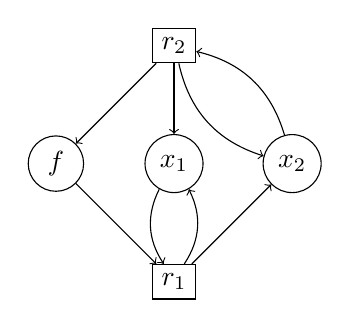
\begin{tikzpicture}
			\node[draw, circle] (f) at (-1.5,0) {$f$};
			
			\node[draw, circle] (x1) at (0,0) {$x_1$};
			\node[draw, circle] (x2) at (1.5,0) {$x_2$};

			\node[draw, rectangle] (r1) at (0,-1.5) {$r_1$};
			\node[draw, rectangle] (r2) at (0,1.5) {$r_2$};
			
			\draw[->] (f) to (r1);
			\draw[->] (r1) to [bend right = 30] (x1);
			\draw[->] (x1) to [bend right = 30] (r1);
			
			\draw[->] (r1) to (x2);
			\draw[->] (x2) to [bend right = 30] (r2);
			\draw[->] (r2) to [bend right = 30] (x2);
			\draw[->] (r2) to (x1);
			\draw[->] (r2) to (f);
		\end{tikzpicture}
	\end{minipage}
	\par\bigskip
	\caption{An irreducible, monocatalyzed RAF $\RAF\coloneqq \{[r_1]_{\sim},[r_2]_{\sim}\}$ as CRN reactions (\textbf{left}) and its K\H{o}nig graph $\king(\RAF)$ (\textbf{right}). }
	\label{fig:foodBlock}
\end{figure}

\holy{We conclude this section by commenting on another property of strong blocks $\block$. The strong connectivity implies that each reaction vertex has at least one incoming edge, from an F-reactant or F-catalyst, and at least one outgoing edge, to an F-catalyst or F-product. Lemma~\ref{lem:StrongBlocks} additionally guarantees that his holds true also for the sub-network $(X(\block)\setminus \food, \CR(\block))$ of $\block$ that is void of food species. Therefore, each reaction has at least one reactant and at least one product. We say that such a sub-network is \emph{well-formed}. 
}





\holy{
Thm.~\ref{Thm:StrBlockCore}  provides only a partial explanation for the large number of autocatalytic cores found e.g. in the examples depicted in Fig.~\ref{fig:irrRAFCores}. It is, therefore, consequential to further investigate the structures of each block that give rise to autocatalytic cores. 


To this end, we revisit the proof of \cite[Thm.~3.1]{golnik_bridging_2026}, where we have shown that each RAF $\RAF$ that is itself not a CAF is associated with an elementary circuit $C$ (SI Sec.~\ref{S-sec:Glossary}) in $\king(\RAF)$, whose species and reaction vertices $X(C)$ and $\CR(C)$, respectively, define an autocatalytic sub-CRN (see also \cite[Remark~13]{golnik_bridging_2026}). We adapt this construction to obtain such an elementary circuit for each strong block.

}

\vspace{6pt}
\begin{lemma}\label{lem:MetzCircuit}
  \holy{Let $\block$ be a maximal, non-trivial strong block of $\king(\RAF)$. Then $\block$ contains an elementary circuit $C$ with one entry reaction for $\block$, and there is a reordering of the columns of $\SM[X(C), R(C)]$ that yields a Metzler matrix.}
\end{lemma}
\begin{proof}
	\holy{We start with the simple case, and assume there is only one reaction $r_1$ in $\block$ satisfying Properties~$i$-$iii.$ of Lemma~\ref{lem:StrongBlocks}. We then have $\crgen(r_1)<\crgen(r)$ for all $r\in \CR(\block) \setminus \{r_1\}$. We may then construct the following elementary circuit:
	\begin{equation}
		r_1 \leftarrow x_1 \leftarrow r_2 \leftarrow x_2 \leftarrow \ldots r_n
		\leftarrow x_m \leftarrow r_{m+1}
	\end{equation}
	such that $x_1$ is an F-catalyst for $r_1$ with the lowest generation order $\sgen(x_1)$ of all F-catalyst of $r_1$, and forall $1< k\leq m+1$: 
	\begin{equation}
		r_k =  \arg \min \{ \crgen(r) \ \vert \ r\in \CR(\block), \SM_{x_{k-1}r}>0\}
	\end{equation}
	and for all $1<k\leq m$:
	\begin{equation}
		x_k = \arg \min \{\sgen(x) \ \vert \ x\in X(\block)\setminus \food, s^-_{xr_k}>0\}.
	\end{equation}
	Since all reactions $r_k, 1< k\leq m$ are not entry reactions vertices, each of them has an F-reactant $x_k$ for which
	$\crgen(r_k)>\sgen(x_k)$ and thereby:
	\begin{equation}
		\crgen(r_k) > \sgen(x_k) \geq \crgen(r_{k+1}), \quad 1< k < m.
	\end{equation}
	$(\crgen(r_k))_{1< k\leq m+1}$ is then a strictly monotone decreasing sequence which converges -- due to the finiteness of $\block$ and positivity of $\beta$ and $\delta$ restricted to the non-food species -- and thereby yields $r_{m+1}=r_1$.  Thus $C\coloneqq (r_{m+1}, x_m, r_m, x_{m-1}, r_{m-1},\ldots, x_1,r_1)$ is an elementary circuit in $\king(\RAF)$.
	
	Assume now that there is $i\neq j$ such that $s^-_{x_ir_j}>0$. If $i>j$ then $\sgen(x_i)<\sgen(x_j)$ which contradicts that $\sgen(x_j)=\min \{\sgen(x) \ \vert \ x\in X(B), s^-_{xr_k}>0\}$. Thus $i<j$, which implies that $\sgen(x_i)\geq\delta(r_j)$ and that $x_i$ cannot be an F-reactant of $r_j$ but only an F-catalyst, thus:
	\begin{equation}
		\SM_{x_ir_j}=0.
	\end{equation} 

	Therefore, the only positive reactant stoichiometries are of the form $s^-_{x_i,r_i}, 1<i\leq m$. We can then obtain $S(C)$ by reordering the columns of the submatrix $\SM[X(C), R(C)]$ such that $S(C)_{x_iy}\coloneqq \SM[X(C), \CR(C)]_{x_ir_i}$. Thereby, all diagonal entries of $\SM(C)$ are nonpositive, $\SM(C)_{x_1r_1}=0$, and all off-diagonal entries of $\SM(C)$ are nonnegative. Thus $\SM(C)$ is a Metzler matrix.
	\vspace{6pt}

	We now turn to the general case and assume there are multiple
	reactions satisfying Properties~$i.$-$iii.$ of Lemma~\ref{lem:StrongBlocks} and we collect them in $R^*(\block)$. We may again choose $r_1\in R^*(\block):
	\crgen(r_1)\leq \crgen(r_j), \forall r_j\in R^*(\block)$ and we have $\crgen(r_1)<\crgen(r), \forall r\in R(\block)\setminus R^*(\block)$. We now apply the same construction as above:
	\begin{equation}
		r_1 \leftarrow x_1 \leftarrow r_2 \leftarrow x_2 \leftarrow \ldots r_n \leftarrow x_m \leftarrow r_{m+1}
	\end{equation}
	such that $x_1$ is an F-catalyst for $r_1$ with the lowest generation order $\sgen(x_1)$ of all F-catalyst of $r_1$, and for all $1< k\leq m+1$:
	\begin{equation}
		r_k = \arg \min \{ \crgen(r) \ | r\in R(\block), \SM_{x_{k-1}>0}\}
	\end{equation}
	and for all $1<k\leq m$:
	\begin{equation}
		x_k = \arg \min \{\delta (x) \ \vert \ x\in X(\block)\setminus\food, s^-_{xr_k}>0\}
	\end{equation}
	if $r_k \notin R^*(\block)$ or $x_k$ as an F-catalyst of $r_k$ otherwise. 
	
	We thereby obtain the following structure:
	\begin{equation*}
		(r_{1,1}, \leftarrow x_{1,1} \leftarrow\ldots \leftarrow x_{1,k_1})
		\leftarrow \ldots \leftarrow (r_{l,1} \leftarrow x_{l,1} \leftarrow
		\ldots \leftarrow x_{l,k_l}) \leftarrow r_{l+1}
	\end{equation*}
	where $r_{1,1} \coloneqq r_1, x_{1,1} \coloneqq x_1$, $r_{l+1}\coloneqq r_{m+1}$ and each reaction vertex $r_{i,1}, 1\leq i\leq l$ is a a reaction $r\in R^*(\block)$, and each species vertex $x_{i,1}, 1\leq i\leq l$ is an F-catalyst for $r_{i,1}$. Then, by the same argument as above, we obtain a strictly monotone decreasing sequence $(\delta(r_{i,j}))_{1\leq j \leq k_i}$ for each $i\in \{1,\ldots l\}$. Again finiteness of $\block$ guarantees 
	$r_{i,1}=r_{l+1}$ for some $i\in \{1,\,\ldots, l\}$, which yields the elementary circuit
	\begin{equation}
		C\coloneqq (r_{l+1}, x_{l,k_l}, \ldots x_{i,1},  r_{i,1}).
	\end{equation}
	Assume now again that we have $i\neq j$ such that $s^-_{x_ir_j}>0$. In the first case, if $x_i, r_j\in (r_{n,1},x_{n,1},\ldots, x_{n,n_k})$ for some $n\in \{1,\ldots, l\}$, we obtain with the same arguments as in the trivial case that $S_{x_ir_j}=0$.

Assume now that there is no such $n$. If $\sgen(x_i)>\sgen(x_j)$ then $\sgen(x_i)\geq \delta(r_j)$ which implies that $x_i$ cannot be an F-reactant for $r_j$, thus $S_{x_ir_j}=0$. The case
$\sgen(x_i)<\sgen(x_j)$ is impossible due to our choice of $x_j$. Then the only remaining case is $\sgen(x_i)=\sgen(x_j)$ which is possible since the minimum of $\{\sgen(x) \ \vert \ x\in X(B), s^-_{xr_j}>0\}$ is not necessarily unique. This, however, implies that there is a smaller elementary circuit containing a reaction from $\CR^*(\block)$. If $i>j$ this circuit can be obtained as $C'$ with:

	\begin{equation}
		\begin{split}
			V(C')&\coloneqq V(C)\setminus \{x_j, r_{j+1}, \ldots, x_{i-1}\}\\[0.5em]
			E(C')& \coloneqq E(C)\setminus \left(\{(x_k, r_k) \ | \ j\leq k < i\} \cup \{(r_k, x_{k-1}) \ | \ j< k \leq i\}\right),
		\end{split}
	\end{equation} 
	or if $i<j$ then this circuit can be obtained as $C'$:
	\begin{equation}
		\begin{split}
			V(C'') & \coloneqq \{x_i, r_{i+1}, \ldots, x_{j-1}, r_{j}\} \\
			E(C'') & \coloneqq\{(x_k, r_k) \ | \ i < k < j\} \cup \{(x_i,r_j)\} \cup \{(r_k, x_{k-1}) \ | \ i < k \leq j\}
		\end{split}
	\end{equation} 
	It holds by construction that either $r_1\in R(C')$ or that there is another reaction $r_{l,1} \in R(C''): i<l\leq j$. We may now repeat
	this procedure until we can not find such a metabolite-to-reaction edge anymore and obtain a final elementary circuit $\tilde{C}$.

	We can then obtain $S(\tilde{C})$ by reordering the columns of the submatrix $\SM[X(\tilde{C}), R(\tilde{C})]$ such that
	\begin{equation}
		\SM(\tilde{C})_{xy}\coloneqq \SM[X(\tilde{C}), R(\tilde{C})]_{xv^{\tilde{C}}_{out}(x)}
	\end{equation} 
	where $v^{\tilde{C}}_{out}(x)$ is the unique reaction $r\in R(\tilde{C})$ such that $(x,r)\in E(\tilde{C})$. Thereby, all diagonal entries of
	$\SM(\tilde{C})$ are nonpositive of which at least one is $0$, and all off-diagonal entries of $\SM(\tilde{C})$ are nonnegative, thus $\SM(\tilde{C})$ is a Metzler matrix.
}
\end{proof}

\vspace{6pt}

\holy{

We call an elementary circuit associated with a stoichiometric Metzler sub-matrix upon suitable column reordering a \emph{Metzler circuit}. Metzler circuits containing an entry reaction for the corresponding block are always \emph{stoichiometrically autocatalytic}.

\vspace{6pt}
\begin{lemma}\label{lem:MetzCircAut}
  Let $\RAF$ be an irreducible, monocatalyzed RAF and $\block$ a maximal, non-trivial strong block of $\king(\RAF)$. Any Metzler circuit $C\subseteq \block$ that contains an entry reaction for $\block$ is \emph{stoichiometrically autocatalytic}.
\end{lemma}
\begin{proof}
	If $C$ is a Metzler circuit that contains a reaction satisfying Properties~$i.$-$iii.$, then there is a reordering of the columns of the stoichiometric submatrix $\SM[X(C),R(C)]$ that reads
	\begin{equation}
		\SM(C) = 
		\begin{pmatrix}
			0 	& 	 		&	 			&  			& 	p_1	\\
			p_2	& 	-r_2  		& 				&     P''  		&		\\
			& 	p_3  		& 	\ddots 		&      			&		\\
			& 	 		& 	\ddots 		& \ddots 		&    	 	\\
			P'	& 	 		& 				& p_k 		& -r_k     	\\
		\end{pmatrix},
	\end{equation}
	with $\{r_i\}\in \mathbb{R}_{\geq 0}, i=2,\ldots, k$ and $\{p_i\}\in \mathbb{R}_{>0},i=1,\ldots, k$ 
	and nonnegative entries in $P'$ and $P''$. We may then construct $v\in \mathbb{R}^{k}_{>0}$ as $v(r_k)\coloneqq 1$ 
	and 
	\begin{equation}
		v_{i}=\begin{cases}
			\frac{v_{i+1}\cdot r_{i+1}}{p_{i+1}} +1 & \text{if } r_{i+1}>0 \\
			\frac{v_{i+1}}{p_{i+1}} +1 & \text{if } r_{i+1}=0
		\end{cases}
	\end{equation}
	Then $v>0$ and by construction we directly obtain $\SM(C)v>0$ since $P'$ and $P''$ contain only nonnegative entries and every row of $S(C)$ contains a strictly positive entry.
\end{proof}
\vspace{6pt}
}
\holy{
\vspace{6pt} Whenever the sub-CRN induced by an elementary circuit $C$ is \emph{stoichiometrically autocatalytic}, we say that $C$ is 
\emph{stoichiometrically autocatalytic}. Metzler circuits can, as shown in the proof of Lemma~\ref{lem:MetzCircuit}, still contain a species-to-reaction or, equivalently, a metabolite-to-reaction (MR-) chord. These chords, however, do not impact the stoichiometric matrix as the involved species is an F-catalyst and the corresponding entry is $0$. The example in Fig.~\ref{fig:RAFContAutCyc} depicts such a scenario. 

\begin{figure}[h]
	\begin{minipage}[c]{0.55\textwidth}
		\begin{equation}
			\begin{split}
				r_1&: f +(x_1) \rightarrow x_2 +(x_1) \\
				r_2&: x_2 + (x_1 + x_2) \rightarrow  x_3 + (x_1 + x_2) \\
				r_3&: x_3 + (x_3) \rightarrow x_1 + (x_3)\\
			\end{split}
		\end{equation}
	\end{minipage}%
	\hfill%
	\begin{minipage}[c]{0.45\textwidth}
		\centering
		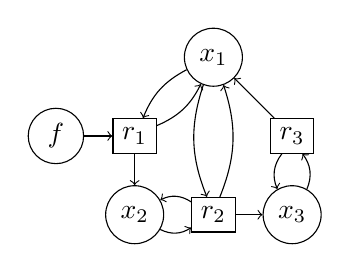
\begin{tikzpicture}
			\node[draw, circle] (f) at (0,0) {$f$};
			\node[draw, circle] (x1) at (2,1) {$x_1$};
			\node[draw, circle] (x2) at (1,-1) {$x_2$};
			\node[draw, circle] (x3) at (3,-1) {$x_3$};
			
			\node[draw, rectangle] (r1) at (1,0) {$r_1$};
			\node[draw, rectangle] (r2) at (2,-1) {$r_2$};
			\node[draw, rectangle] (r3) at (3,0) {$r_3$};
			
			\draw[->] (f) to (r1);
			\draw[->] (x1) to [bend right = 20] (r1);
			\draw[->] (r1) to [bend right = 20] (x1);
			\draw[->] (r1) to (x2);
			\draw[->] (r2) to [bend right = 20] (x1);
			\draw[->] (x1) to [bend right = 20] (r2);
			\draw[->] (x2) to [bend right = 30] (r2);
			\draw[->] (r2) to [bend right = 30] (x2);
			\draw[->] (r2) to (x3);
			\draw[->] (r3) to (x1);
			\draw[->] (x3) to [bend right = 30] (r3);
			\draw[->] (r3) to [bend right = 30] (x3);
		\end{tikzpicture}
	\end{minipage}
	\caption{Example of a non-trivial, irreducible RAF with three reactions on four species vertices, where the spanning autocatalytic Metzler circuit as constructed by the proof of Lemma~\ref{lem:MetzCircuit} is not an autocatalytic core.}
	\label{fig:RAFContAutCyc}
\end{figure}


Elementary circuits free of MR-chords play an important role in enumerating autocatalytic cores \cite{golnik_using_2026}. As they are always Metzler circuits, the following corollary is a direct consequence of Lemma~\ref{lem:MetzCircuit}.
\vspace{6pt}
\begin{corollary}\label{cor:MRChordlessAutocat}
  Any MR-chordless elementary circuit $C$ of a maximal, non-trivial strong block $\block$ containing an entry reaction for $\block$ is autocatalytic.
\end{corollary}
\vspace{6pt}
}

\holy{
In case the maximal strong block $\block$ consists of a single reaction $r$ and a single species $x\notin \food$, Lemma~\ref{lem:StrongBlocks} guarantees $x$ is being an F-catalyst and an F-product at the same time. In addition, there is only one elementary circuit, in particular, the digon $(x,r,x)$, which is by definition a Metzler circuit.
\vspace{6pt}
\begin{corollary}\label{cor:AutoCatReac}
  Let $\RAF$ be an irreducible, monocatalyzed RAF and $\block$ a maximal strong block of $\king(\RAF)$. If $|\CR(\block)|=|X(\block)|=1$ and $X(\block)\cap \food=\emptyset$, then $r$ is an autocatalytic reaction.
\end{corollary}
\vspace{6pt}

The following example illustrates such a situation. 
\begin{figure}[h]
  \centering
  \begin{minipage}[c]{0.5\textwidth}
    \begin{equation}
      \begin{split}
	r_1&: f + (x_1) \rightarrow x_2 + (x_1) \\
	r_2&: 2x_2 + (x_3) \rightarrow x_4 + x_3 +(x_3) \\
	r_3&: x_4 + (x_4) \rightarrow x_1 + (x_4)
      \end{split}
    \end{equation}
  \end{minipage}%
  \hfill%
  \begin{minipage}[c]{0.5\textwidth}
    \centering
    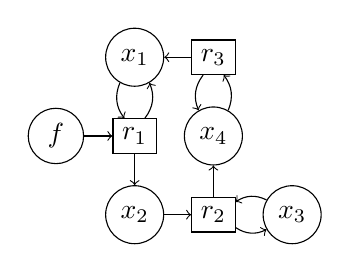
\begin{tikzpicture}
      \node[draw, circle] (f) at (0,0) {$f$};
      \node[draw, circle] (x1) at (1,1) {$x_1$};
      \node[draw, circle] (x2) at (1,-1) {$x_2$};
      \node[draw, circle] (x3) at (3,-1) {$x_3$};
      \node[draw, circle] (x4) at (2,0) {$x_4$};
      
      \node[draw, rectangle] (r1) at (1,0) {$r_1$};
      \node[draw, rectangle] (r2) at (2,-1) {$r_2$};
      \node[draw, rectangle] (r3) at (2, 1) {$r_3$};
      
      \draw[->] (f) to (r1);
      \draw[->] (x1) to [bend right = 30] (r1);
      \draw[->] (r1) to [bend right = 30] (x1);
      \draw[->] (r1) to (x2);
      \draw[->] (x2) to (r2);			
      \draw[->] (x4) to [bend right = 30] (r3);
      \draw[->] (r3) to [bend right = 30] (x4);
      \draw[->] (r2) to (x4);
      \draw[->] (x3) to [bend right = 30] (r2);
      \draw[->] (r2) to [bend right = 30] (x3);
      \draw[->] (r3) to (x1);
    \end{tikzpicture}
  \end{minipage}
  \caption{An irreducible, monocatalyzed RAF with an autocatalytic reaction $r_2$.}
  \label{Fig:ExplAutocatReac}
\end{figure}
\FloatBarrier Indeed, $\block\coloneqq \{x_3, r_2\}$ is a maximal strong block and $r_2$ is an autocatalytic reaction.
}

\holy{Lemma~\ref{lem:MetzCircuit}, \ref{lem:MetzCircAut}, and
Cor.~\ref{cor:AutoCatReac}, together, yield the following main result.

\vspace{6pt}
\begin{theorem}\label{thm:mainsecond}
  Let $\RAF$ be an irreducible, monocatalyzed RAF. Then every maximal, non-trivial strong block $\block$ of $\king(\RAF)$ contains an autocatalytic Metzler circuit. If $V(\block)=\{x,r\}$ such that $x\notin \food$, $r$ is an autocatalytic reaction.
\end{theorem} 
\vspace{6pt}

The autocatalytic elementary circuits, as constructed in the proof of Lemma~\ref{lem:MetzCircuit}, are not necessarily cores for various reasons. One is MR-chords that appear as digons, i.e., elementary circuits of length $2$ whose species-to-reaction edge is not located along the original Metzler circuit (Fig.~\ref{fig:RAFContAutCyc}). Another reason is non-unit stoichiometries, which can give rise to strictly smaller circuits inside the constructed \emph{stoichiometrically autocatalytic} Metzler circuit (Fig.~\ref{fig:NonUnStoich}). As the K\H{o}nig graph is a simple digraph, stoichiometries are naturally not encoded besides being specified as edge labels. As in \cite{golnik_autocatalytic_2026}, we can, therefore, not hope to find a general construction method that identifies autocatalytic cores directly.

\begin{figure}[htb]
	\begin{minipage}[c]{0.5\textwidth}
		\begin{equation}
			\begin{split}
				r_1&: f + (x_1) \rightarrow x_2 + (x_1) \\
				r_2&: x_2 + (x_2) \rightarrow x_3 + (x_2) \\
				r_3&: x_3 + (x_3) \rightarrow x_1 + 2x_2 + (x_3) 				  
			\end{split}
		\end{equation}
	\end{minipage}%
	\hfill%
	\begin{minipage}[c]{0.5\textwidth}
		\centering
		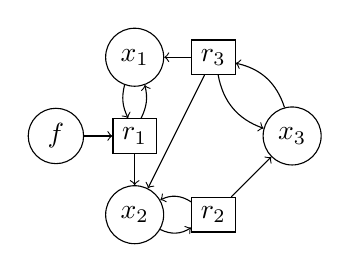
\begin{tikzpicture}
			\node[draw, circle] (f) at (0,0) {$f$};
			\node[draw, circle] (x1) at (1,1) {$x_1$};
			\node[draw, circle] (x2) at (1,-1) {$x_2$};
			\node[draw, circle] (x3) at (3,0) {$x_3$};
			
			\node[draw, rectangle] (r1) at (1,0) {$r_1$};
			\node[draw, rectangle] (r2) at (2,-1) {$r_2$};
			\node[draw, rectangle] (r3) at (2,1) {$r_3$};
			
			\draw[->] (f) to (r1);
			\draw[->] (x1) to [bend right = 20] (r1);
			\draw[->] (r1) to [bend right = 20] (x1);
			\draw[->] (r1) to (x2);
			\draw[->] (x2) to [bend right = 30] (r2);
			\draw[->] (r2) to [bend right = 30] (x2);			
			\draw[->] (r2) to(x3);			
			\draw[->] (x3) to [bend right = 30] (r3);
			\draw[->] (r3) to [bend right = 30] (x3);
			\draw[->] (r3) to (x1);
			\draw[->] (r3) to (x2);			
		\end{tikzpicture}
	\end{minipage}
	\caption{Example of an irreducible, monocatalyzed RAF that contains an autocatalytic core $\{x_2,r_2,x_3,r_3\}$ with non-unit stoichiometries, that would not be constructed by the proof of Lemma~\ref{lem:MetzCircuit} as it would return the autocatalytic
	Metzler circuit $C\coloneqq (r_1,x_2,r_2,x_3,r_3,x_1,r_1)$}
	\label{fig:NonUnStoich}
\end{figure}

However, each maximal, non-trivial strong block $\block$ of the K\H{o}nig graph representation of an irreducible, monocatalyzed RAF $\RAF$ contains an autocatalytic core (Thm.~\ref{Thm:StrBlockCore}), which is a strongly connected subgraph \cite{golnik_autocatalytic_2026} of an autocatalytic elementary circuit $C$ (Lemmata~\ref{lem:MetzCircuit} and \ref{lem:MetzCircAut}). Since every strongly connected subgraph of $\king(\RAF)[X(C)\cup \CR(C)]$ is \emph{Hamiltonian} \cite{bang-jensen_digraphs_2002} -- which means that it encompasses an elementary circuit passing each vertex, also referred to as a \emph{spanning circuit} -- each autocatalytic core derived in this way is Hamiltonian. If the core contains an entry reaction for $\block$, Cor.~\ref{cor:MRChordlessAutocat} in combination with the minimality of autocatalytic cores yields that the spanning circuit is free of reaction-to-metabolite (RM)-chords except for the digon-induced one that connects the entry reaction to its F-catalyst.

\vspace{6pt}
\begin{proposition}\label{Prop:OneCircCorePerBlock}
	Let $\RAF$ be an irreducible, monocatalyzed RAF. Every maximal, non-trivial strong block $\block$ of $\king(\RAF)$ contains an autocatalytic core $(\tilde{X},\tilde{\CR})$ whose induced subgraph $G\coloneqq\king(\RAF)[\tilde{X}\cup \tilde{\CR}]$ is Hamiltonian. If there is an entry reaction for $\block$ s.t. $r\in \tilde{\CR}$, $G$ is an elementary circuit with exactly one RM-chord $(r,x)$, where $x$ is the F-catalyst of $r$. 
\end{proposition}
\vspace{6pt}
}

\holy{Finally, we shed light on the unexpectedly large number of autocatalytic cores associated with each irreducible RAF in random instances of the binary polymer model, as shown in Fig.~\ref{fig:irrRAFCores}. Every autocatalytic core can be considered an element of an equivalence class w.r.t. the relation: 
\begin{equation}\label{eq:CoreEquiv}
	(X_1,\CR_1)\simeq (X_2,\CR_2) \Leftrightarrow X_1=X_2, \exists \lambda: \CR_1\rightarrow \CR_2, \text{ s.t. } [r]_{\mathord{\sim}}=[\lambda(r)]_{\mathord{\sim}}, \forall r\in \CR_1
\end{equation}
with $\sim$ as defined in Eq.~\eqref{eq:EqRel}. Accordingly, each reaction $r$, whose unique incoming edge (\emph{fluffle} property~F3) originates from an F-reactant of $r$, can be substituted by any $r'\in [r]_\sim$, ensuring that the modified sub-CRN exists in $\Gamma(\CRS)$, is autocatalytic, and is an element of the same $\simeq$-equivalence class. 

\vspace{6pt}
\begin{proposition}\label{prop:ExpoNoCores}
	Let $\mathbf{\Phi}\coloneqq (X, \FR, \cat(\FR))$ be a CRS with specified food-set $\food$, $\RAF$ an irreducible RAF, $(\tilde{X},\tilde{\CR})$ an autocatalytic core in $\Gamma(\mathbf{\Phi})
	$, and 
	\begin{equation}
		\tilde{\CR}_F\coloneqq \{r\in \tilde{\CR} \ \vert \ \forall x\in X: s^-_{xr} \Rightarrow \sigma^-_{xr}>0 \}.
	\end{equation}
	Then it holds that
	\begin{equation}\label{eq:NoEquivAutoCatCycles}
		|[(\tilde{X}, \tilde{\CR})]|_{\mathord{\simeq}} = \prod_{r\in\tilde{\CR}_F}|[r]_{\mathord{\sim}}|.
	\end{equation}
\end{proposition}
\vspace{6pt}

Unfortunately, not every element of a $\simeq$-equivalence class is necessarily a core, as the following example illustrates:

\begin{figure}[htb]
	\centering
	\begin{minipage}[c]{0.5\textwidth}
		\begin{equation}
			\begin{split}
				r_1: f + (x_1) \rightarrow x_2 + x_4 + (x_1) \\[0.5em]
				r'_2: x_2 + (x_1) \rightarrow x_2 + x_3 + (x_1) \\[0.5em]
				r''_2: x_2 + (x_4) \rightarrow x_2 + x_3 + (x_4) \\[0.5em]
				r_3: x_3 + (x_3) \rightarrow x_1 + (x_3)				
			\end{split}			
		\end{equation}
	\end{minipage}%
	\hfill%
	\begin{minipage}[c]{0.5\textwidth}
		\centering
		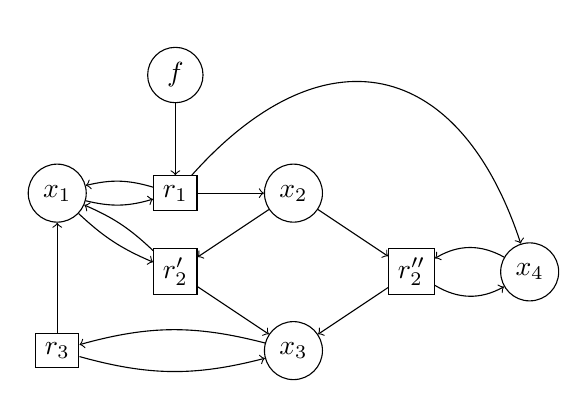
\begin{tikzpicture}
			\node[draw, circle] (f) at (1.5,1.5) {$f$};		
			\node[draw, circle] (x1) at (0,0) {$x_1$};
			\node[draw, circle] (x2) at (3,0) {$x_2$};
			\node[draw, circle] (x3) at (3,-2) {$x_3$};
			\node[draw, circle] (x4) at (6,-1) {$x_4$};	
			
			\node[draw, rectangle] (r1) at (1.5,0) {$r_1$};
			\node[draw, rectangle] (r2') at (1.5,-1) {$r'_2$};
			\node[draw, rectangle] (r2'') at (4.5,-1) {$r''_2$};
			\node[draw, rectangle] (r3) at (0,-2) {$r_3$};
			
			\draw[->] (f) to (r1);
			\draw[->] (x1) to [bend right = 15] (r1);
			\draw[->] (r1) to [bend right = 15] (x1);			
			\draw[->] (r1) to (x2);
			\draw[->] (r1) to [bend left = 60, looseness = 1.5] (x4);
			
			\draw[->] (x2) to (r2');
			\draw[->] (x2) to (r2'');
			
			\draw[->] (x1) to [bend right = 10] (r2');
			\draw[->] (r2') to [bend right = 10] (x1);			
			\draw[->] (x4) to [bend right = 30] (r2'');
			\draw[->] (r2'') to [bend right = 30] (x4);
			
			\draw[->] (r2') to (x3);
			\draw[->] (r2'') to (x3);
			
			\draw[->] (x3) to [bend right = 15] (r3);
			\draw[->] (r3) to [bend right = 15] (x3);
			
			\draw[->] (r3) to (x1);

		\end{tikzpicture}
	\end{minipage}
	\caption{Illustration of CRN reactions (\textbf{left}) and the bipartite K\H{o}nig graph (\textbf{right}) of an irreducible RAF in which two catalyzations for one F-reaction influence minimality of an autocatalytic subsystem and give rise to two distinct autocatalytic cores of different size.}
	\label{fig:Minimality}
\end{figure}

While $(\{x_1, x_2, x_3\}, \{r_1,r_2'', r_3\})$ is an autocatalytic core, $(\{x_1, x_2, x_3\}, \{r_1,r_2', r_3\})$ is not, since the F-catalyst $x_1$ of $r'_2$ induces an MR-chord. In this case $(\{x_1,x_3\}, \{r'_2, r_3\})$ is the autocatalytic core. It becomes evident that the minimality of autocatalytic cores in irreducible RAFs is dependent on the catalyzation. Eq.\eqref{eq:NoEquivAutoCatCycles} then only informs on an upper bound for the number of autocatalytic cores in each $\simeq$-equivalence class. The number of autocatalytic cores in $\Gamma(\CRS)$ scales with the number of $\simeq$ equivalence classes. 

Cores in the same equivalence class support self-sustainability for an identical set of species; however, they can achieve this through different combinations of catalyzations, of which there may be exponentially many. In contrast to the number of autocatalytic cores in each irreducible RAF, the number of equivalence classes is, indeed, tremendously reduced (Fig.~\ref{fig:UniqueFReactionCores}). Still, as each of the depicted irreducible RAFs consists of exactly one maximal, non-trivial strong block, additional cores that are not captured by the constructive results (Lemmata~\ref{lem:MetzCircuit} and ~\ref{lem:MetzCircAut}) still exist.
}

\begin{figure}[htb]
	\centering
	\begin{minipage}[c]{\textwidth}
		\begin{minipage}[c]{0.5\textwidth}
			\centering
			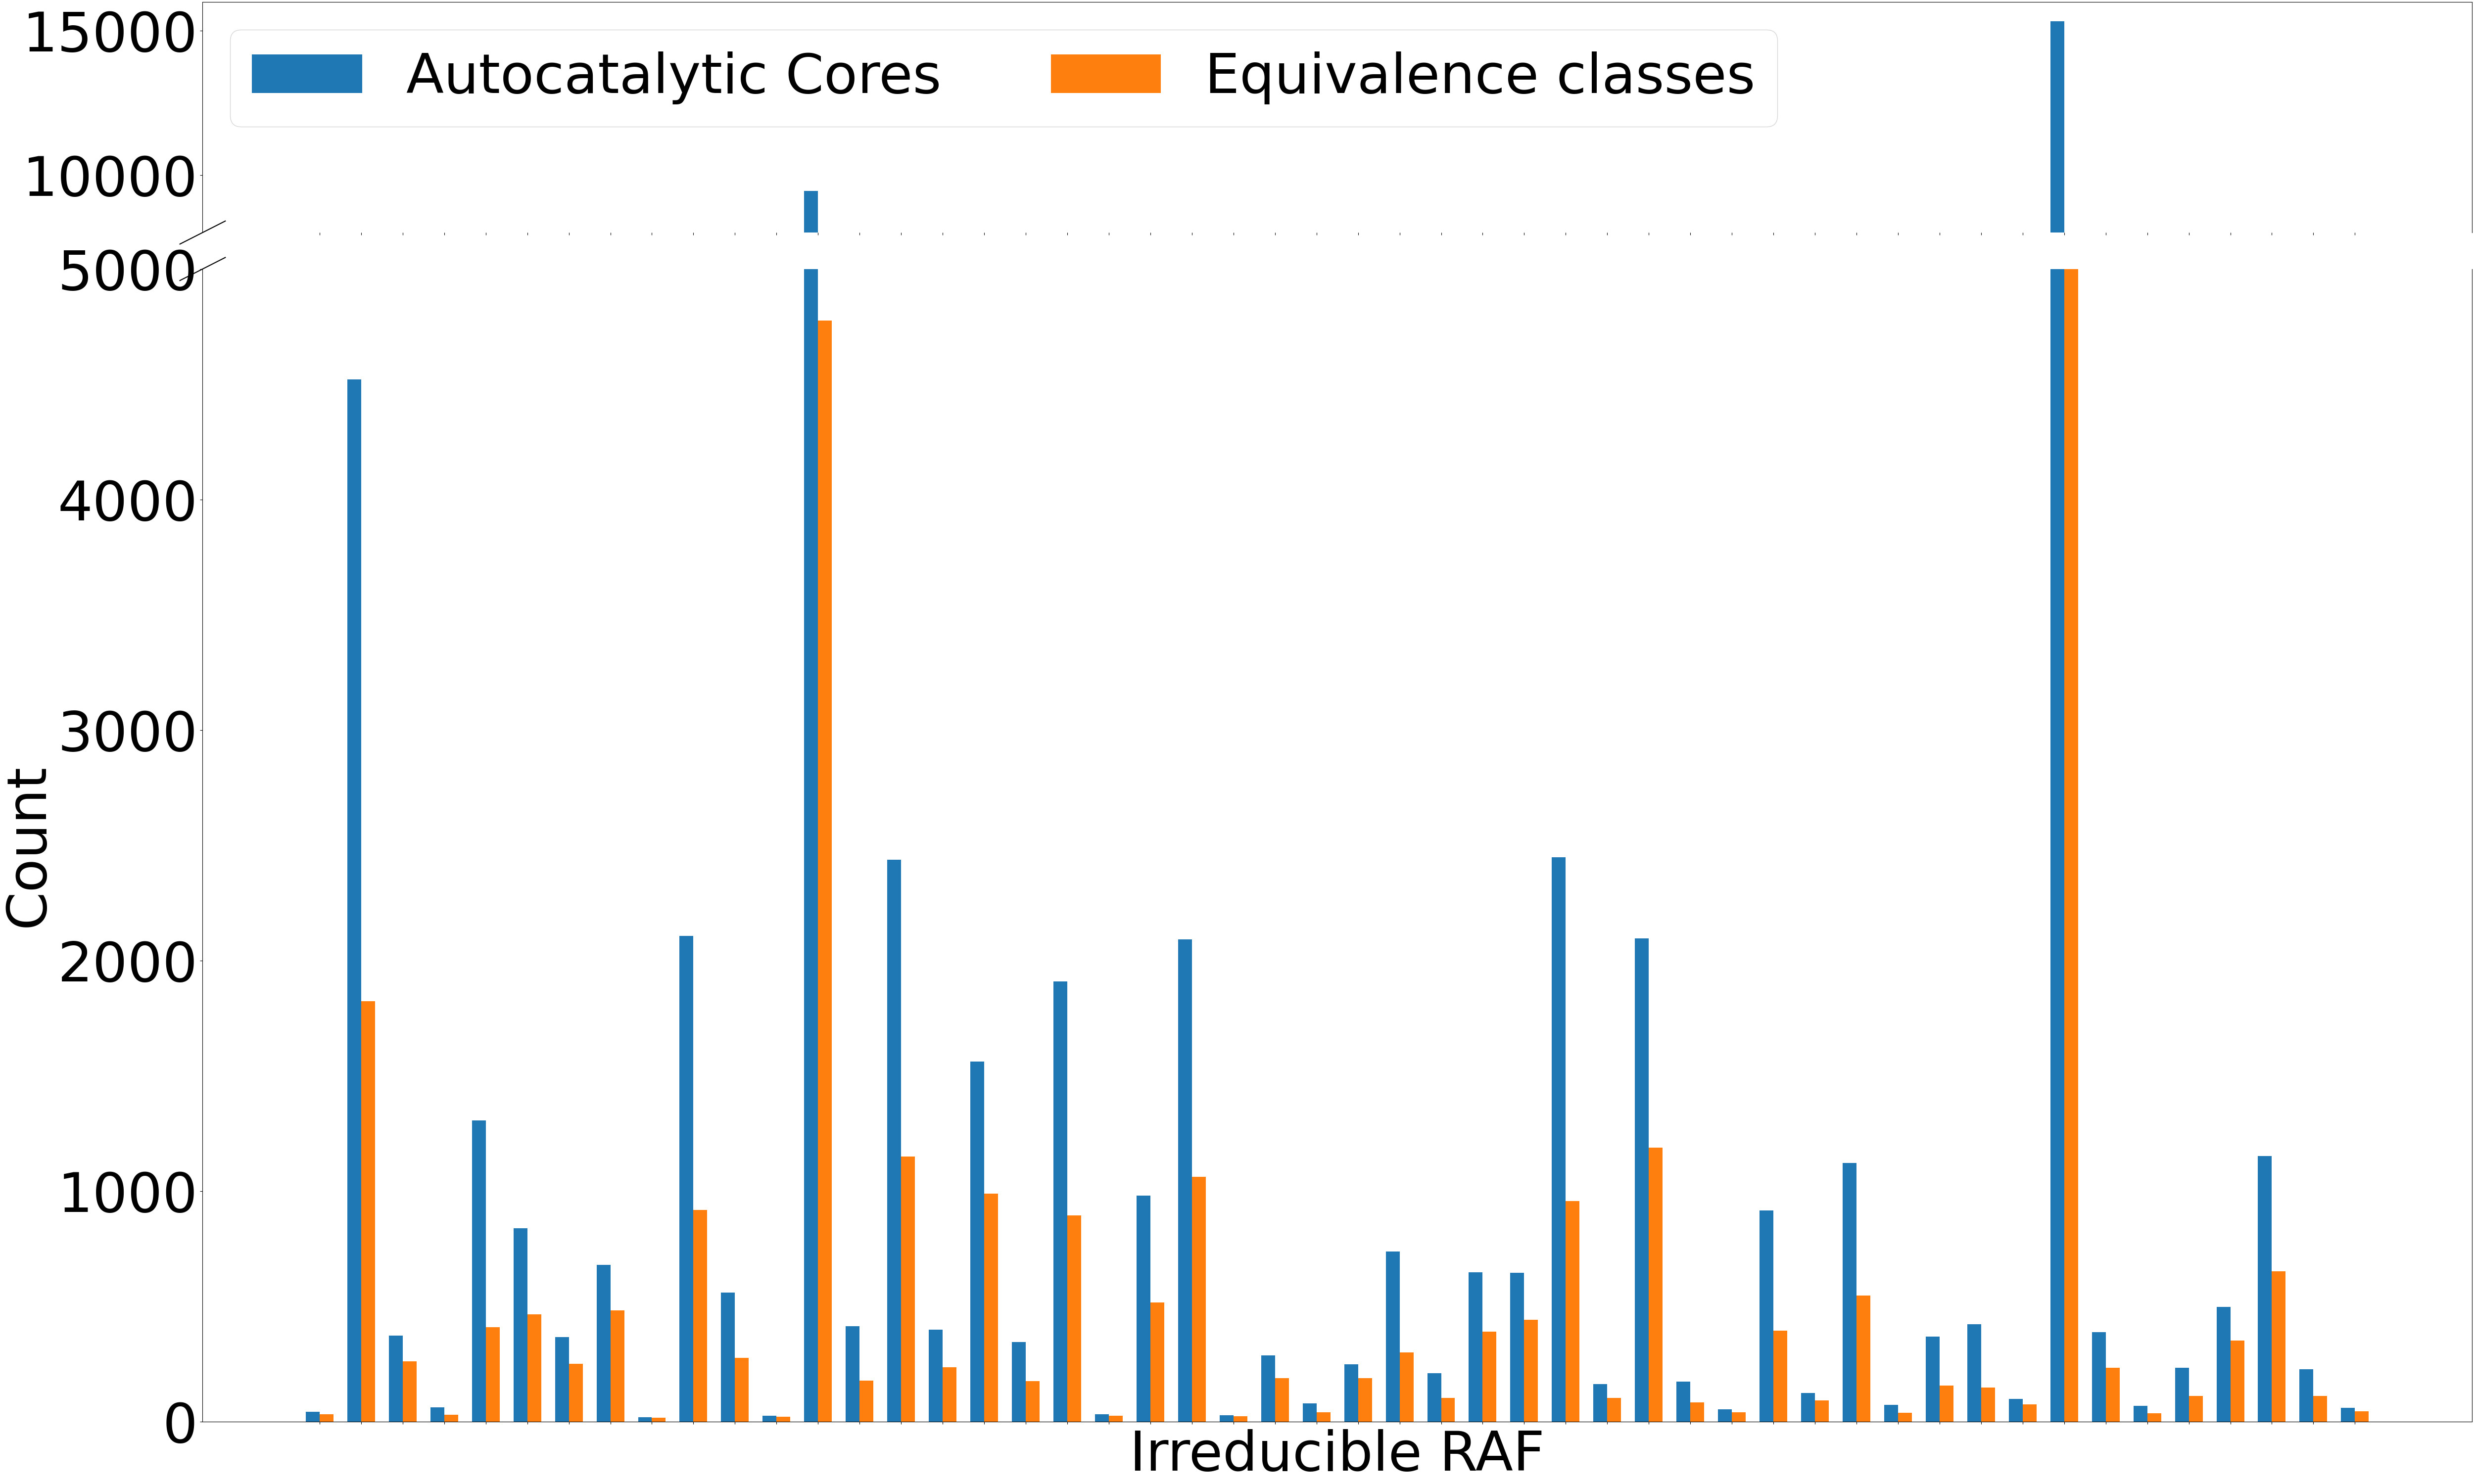
\includegraphics[width=\textwidth]{./Pictures/UniqueFReactionCoresn5rev.png}
		\end{minipage}%
		\hfill%
		\begin{minipage}[c]{0.5\textwidth}
			\centering
			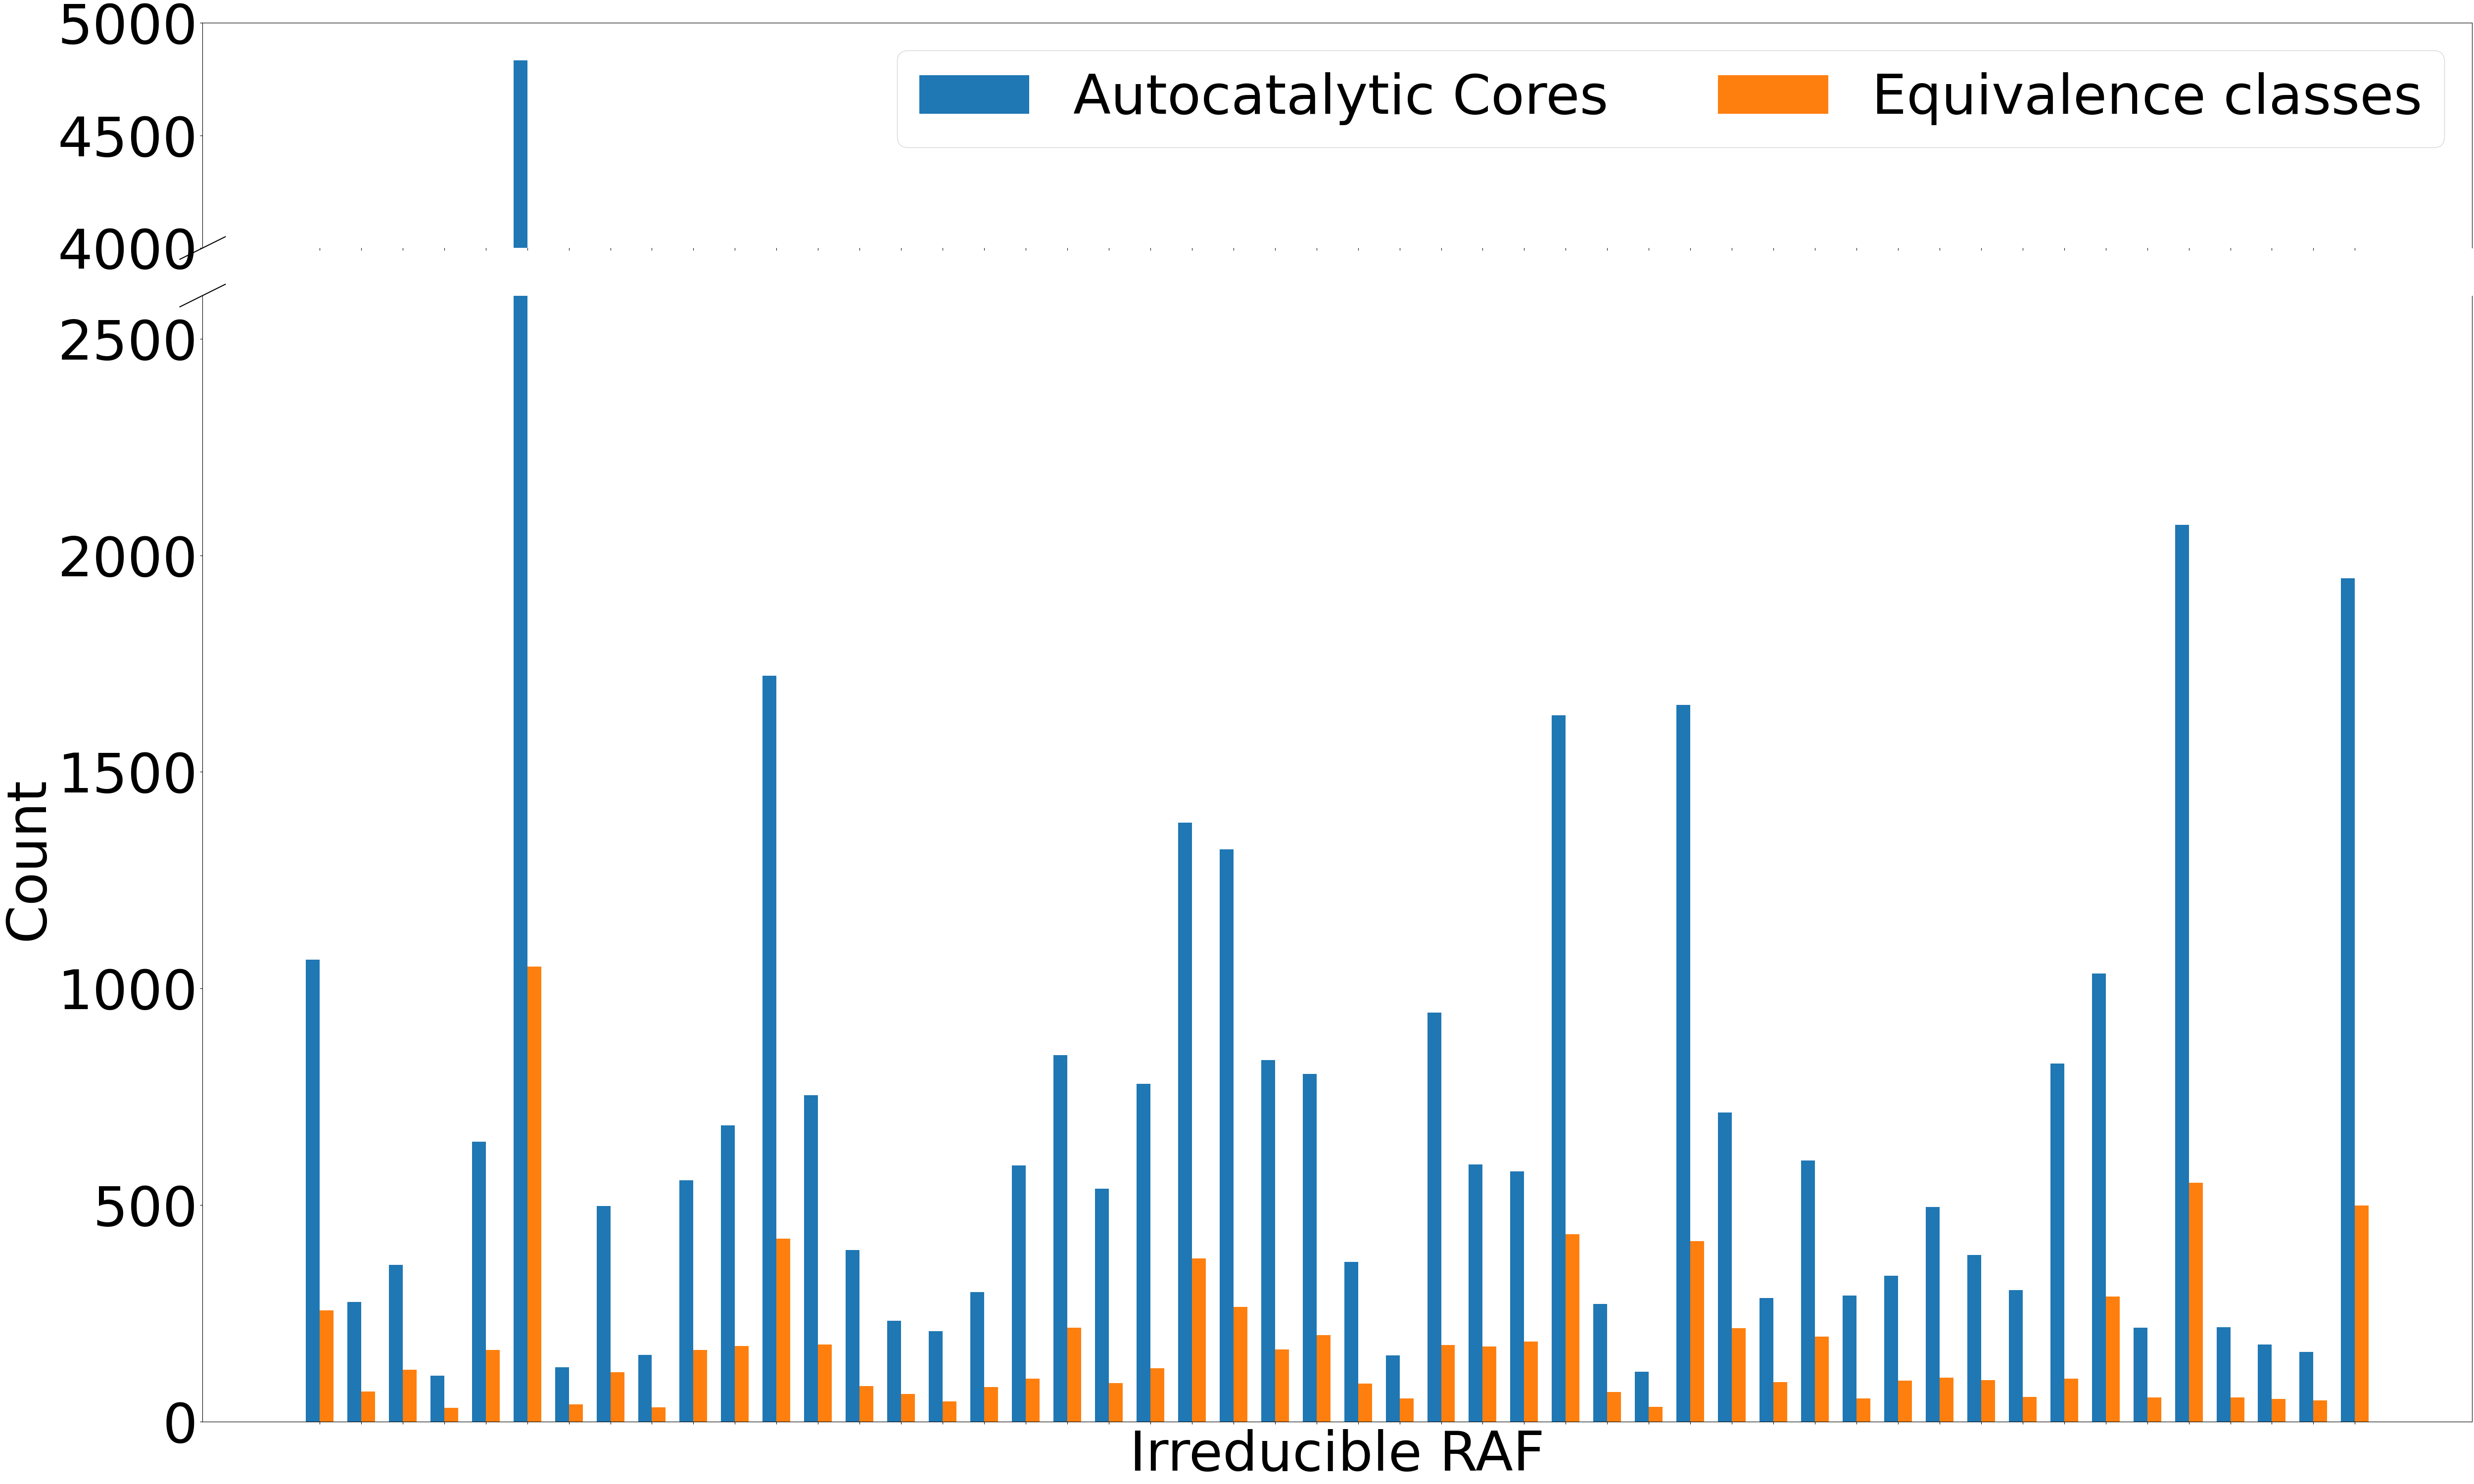
\includegraphics[width=\textwidth]{./Pictures/UniqueFReactionCoresn5rev2.png}
		\end{minipage}
	\end{minipage}
	\begin{minipage}[c]{\textwidth}
		\begin{minipage}[c]{0.5\textwidth}
			\centering
			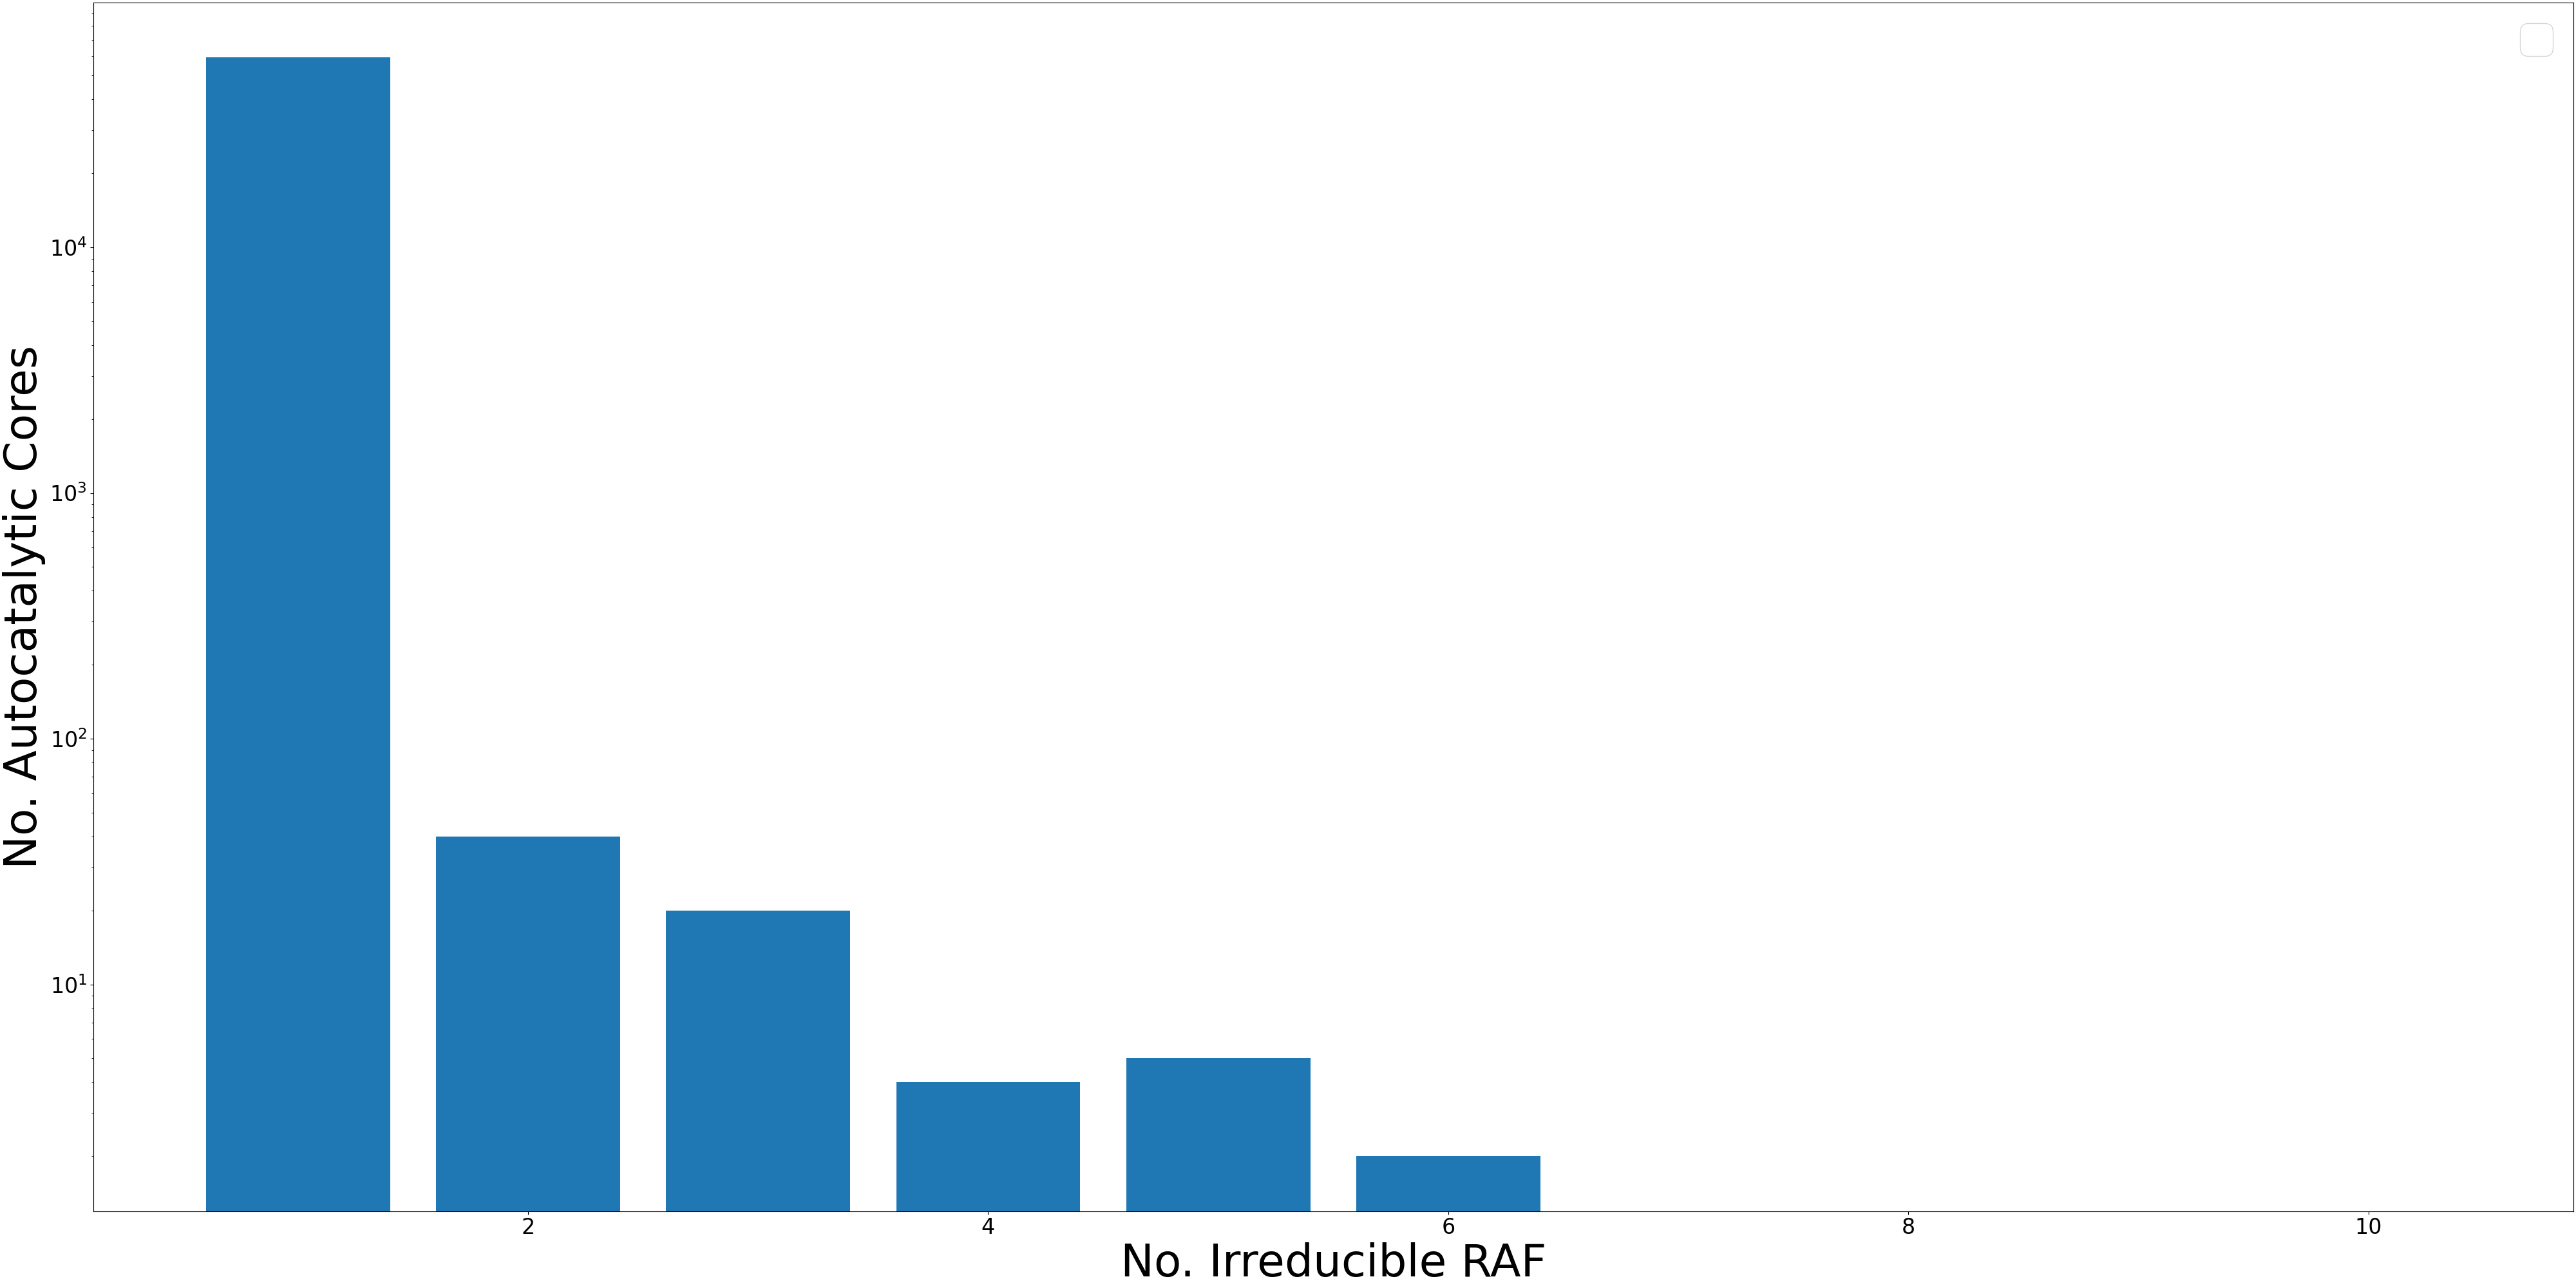
\includegraphics[width=\textwidth]{./Pictures/CoreReusageIrrRAFn5rev.png}
		\end{minipage}%
		\hfill%
		\begin{minipage}[c]{0.5\textwidth}
			\centering
			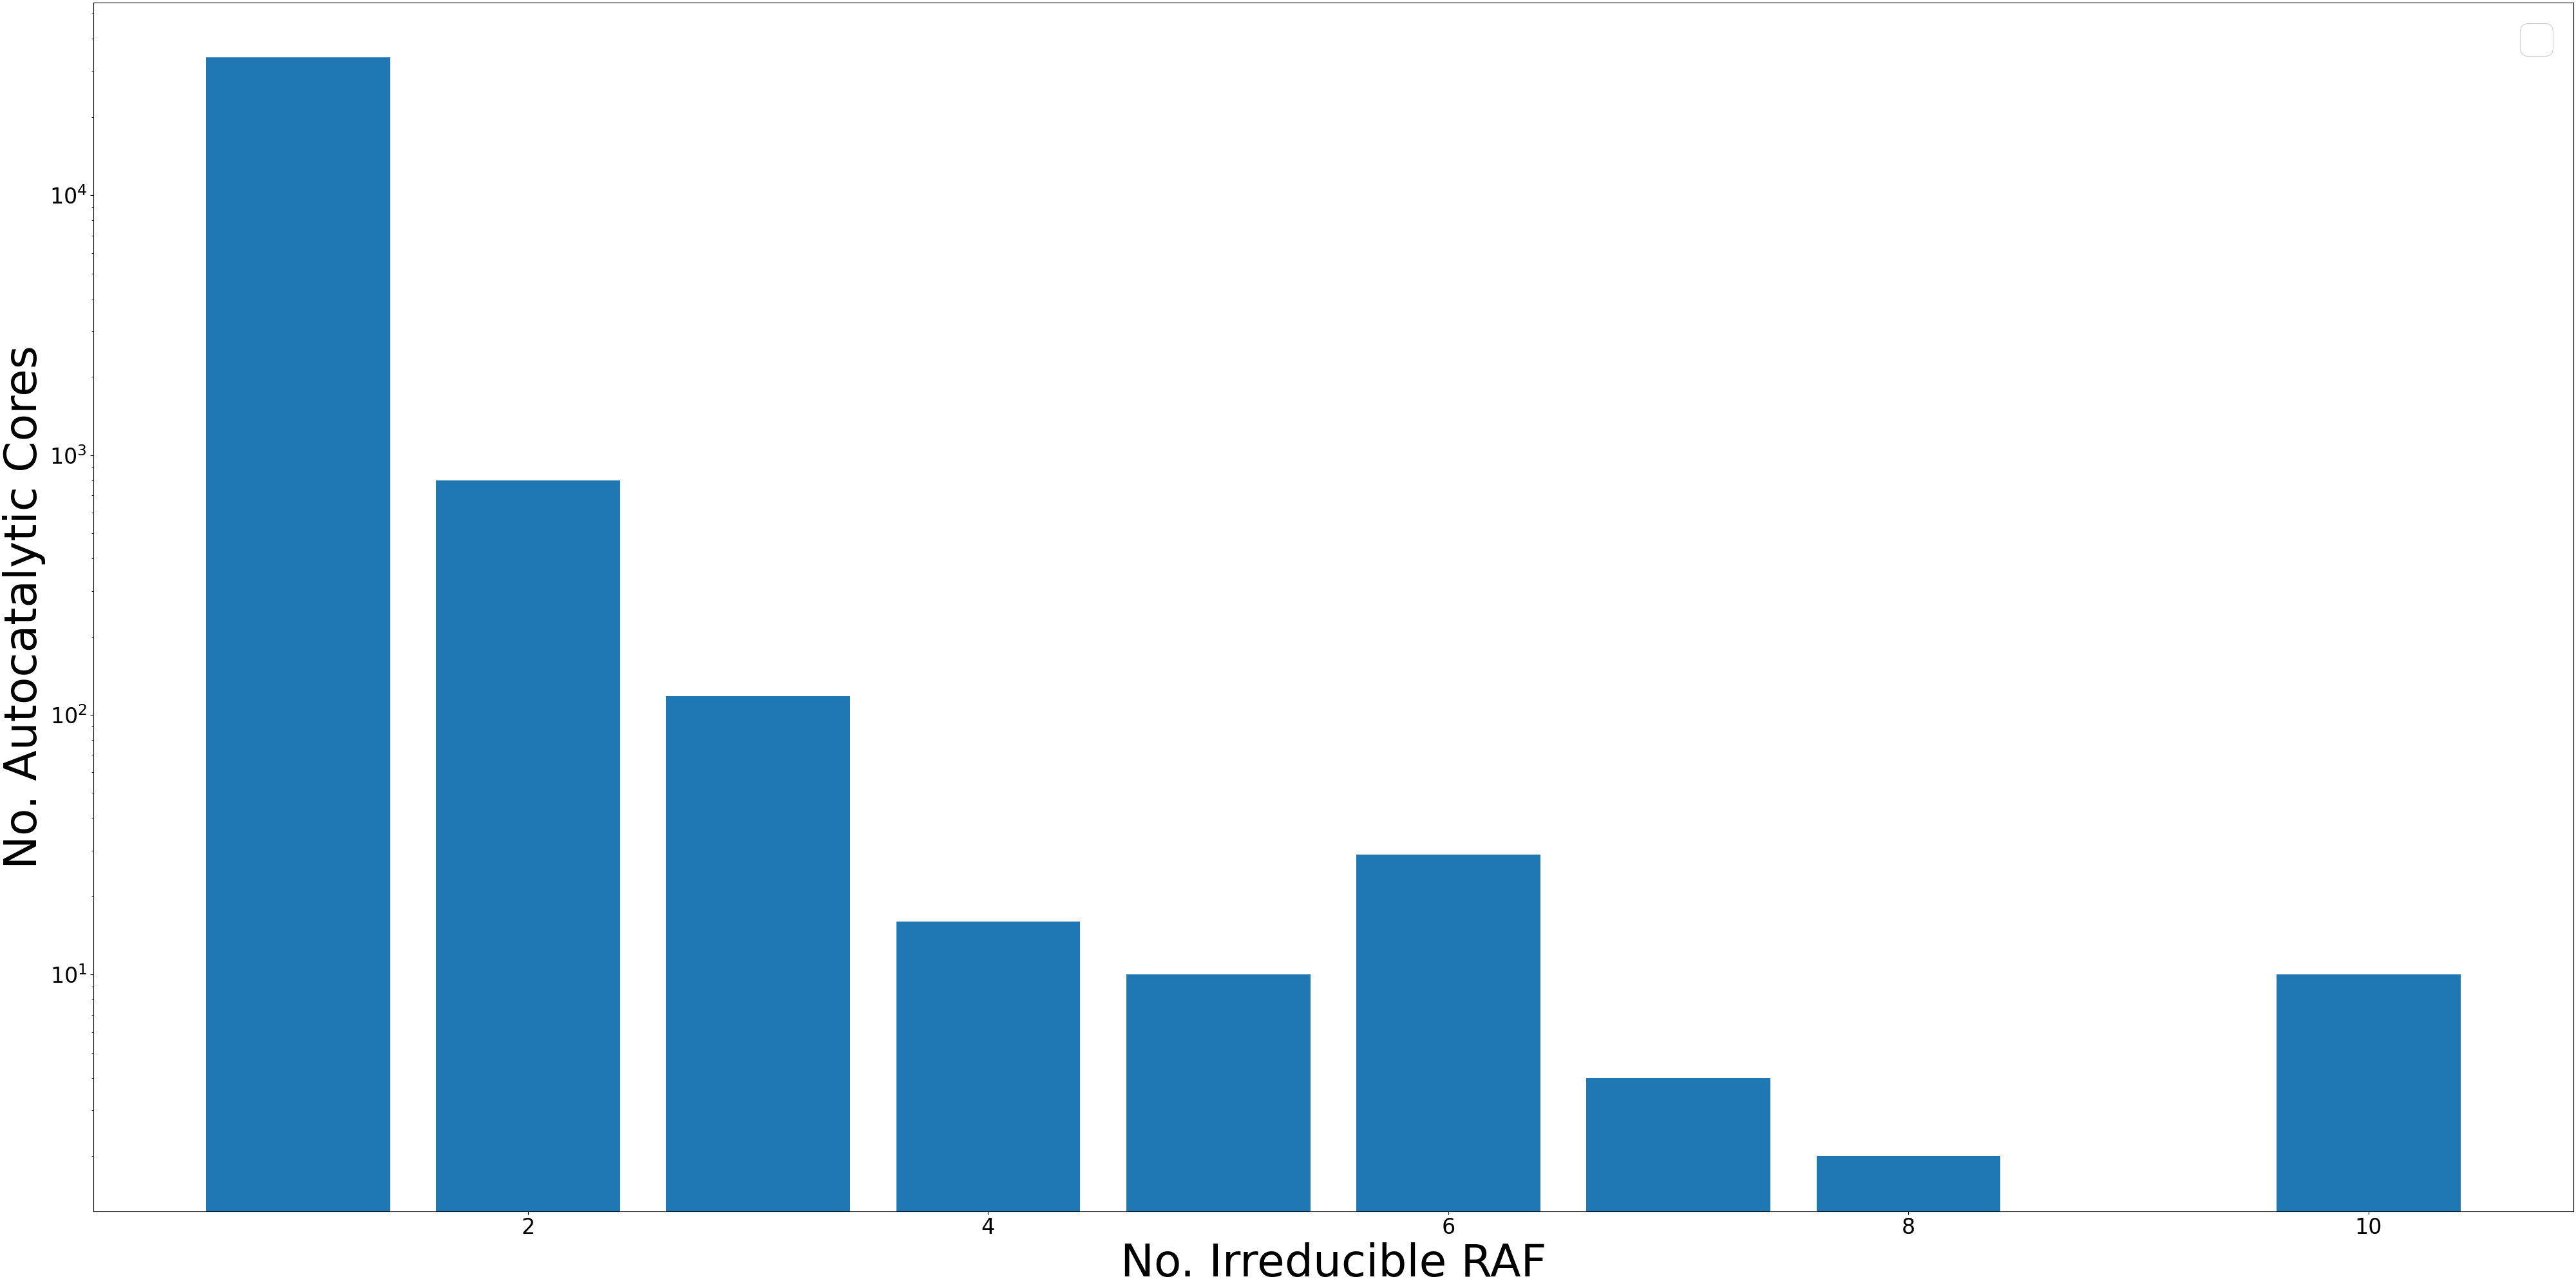
\includegraphics[width=\textwidth]{./Pictures/CoreReusageIrrRAFn5rev2.png}
		\end{minipage}	
	\end{minipage}
	\caption{\textbf{Upper:} Number of autocatalytic cores and autocatalytic core equivalence classes according 
		to Eq.~\eqref{eq:CoreEquiv} among non-food molecules in 50 different irreducible RAFs from 
		two random instances of the binary polymer model with a fixed probability for any non-food 
		species to catalyze any reaction of $p=0.01$ (\textbf{right}) and $p=0.008$ (\textbf{left}) and 
		maximum polymer-length $5$. \textbf{Lower:} Appearance of autocatalytic cores in irreducible 
		RAFs. }
	\label{fig:UniqueFReactionCores}
\end{figure}

\bibliography{RAFCores}

\end{document}
